\documentclass[tikz]{standalone}

\usepackage[T1]{fontenc}
\usepackage[english]{babel}

\usepackage{tikz}

\begin{document}

	\begin{tikzpicture}
		\node[visible on=<1>] (image) {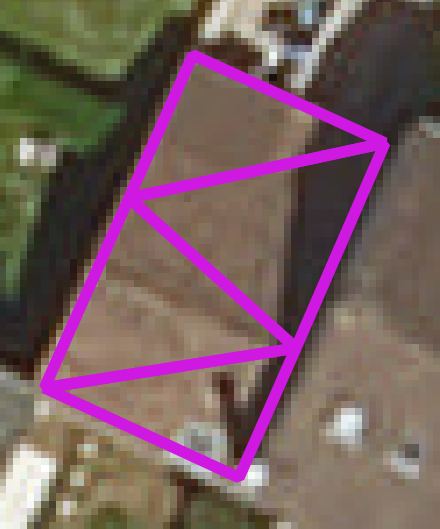
\includegraphics[width=1.5cm, angle=270]{images/introduction/graphical_abstract/orthoprojection}};
		\path (image.south) node[anchor=north, visible on=<1>, text width=1.5cm] (image_legend) {\scriptsize Nadir projection on orthoimage.};

		\path (image) node[visible on=<2>] (pixel_segment) {\includestandalone[width=1.5cm]{figures/features/image_based}};

		\path (image) node[visible on=<3->] (segment_hist) {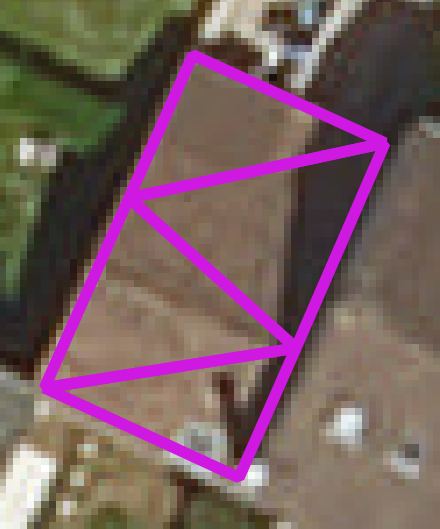
\includegraphics[width=1.5cm, angle=270]{images/introduction/graphical_abstract/orthoprojection}};

		\path (image) + (.7, -.3) node[visible on =<3>] (segment_hist_1) {
			\resizebox{.25cm}{.25cm}{
				\begin{tikzpicture}background rectangle/.style={fill=white}, show background rectangle
					\begin{axis}[
						area style,
						axis background/.style={fill=white},
						ymin=0,
						ytick=\empty,
						xtick=\empty,
						visible on=<3>
					]
						\addplot+[ycomb, blue, mark=*, mark options={scale=2, fill=blue}, very thick] plot coordinates {
							(-8, 3623)
							(-7, 546)
							(-6, 159)
							(-5, 182)
							(-4, 70)
						};
					\end{axis}
				\end{tikzpicture}
			}
		};
		\path (image) + (-.65, .35) node[visible on =<3>] (segment_hist_2) {
			\resizebox{.25cm}{.25cm}{
				\begin{tikzpicture}background rectangle/.style={fill=white}, show background rectangle
					\begin{axis}[
						area style,
						axis background/.style={fill=white},
						ymin=0,
						ytick=\empty,
						xtick=\empty,
						visible on=<3>
					]
						\addplot+[ycomb, blue, mark=*, mark options={scale=2, fill=blue}, very thick] plot coordinates {
							(-8, 3623)
							(-7, 546)
							(-6, 1595)
							(-5, 182)
							(-4, 4151)
						};
					\end{axis}
				\end{tikzpicture}
			}
		};
		\path (image) + (-.6, -.25) node[visible on =<3>] (segment_hist_3) {
			\resizebox{.25cm}{.25cm}{
				\begin{tikzpicture}background rectangle/.style={fill=white}, show background rectangle
					\begin{axis}[
						area style,
						axis background/.style={fill=white},
						ymin=0,
						ytick=\empty,
						xtick=\empty,
						visible on=<3>
					]
						\addplot+[ycomb, blue, mark=*, mark options={scale=2, fill=blue}, very thick] plot coordinates {
							(-8, 3623)
							(-7, 5446)
							(-6, 159)
							(-5, 1852)
							(-4, 70)
						};
					\end{axis}
				\end{tikzpicture}
			}
		};
		\path (image) + (.1, -.5) node[visible on =<3>] (segment_hist_4) {
			\resizebox{.25cm}{.25cm}{
				\begin{tikzpicture}background rectangle/.style={fill=white}, show background rectangle
					\begin{axis}[
						area style,
						axis background/.style={fill=white},
						ymin=0,
						ytick=\empty,
						xtick=\empty,
						visible on=<3>
					]
						\addplot+[ycomb, blue, mark=*, mark options={scale=2, fill=blue}, very thick] plot coordinates {
							(-8, 3623)
							(-7, 546)
							(-6, 159)
							(-5, 182)
							(-4, 5670)
						};
					\end{axis}
				\end{tikzpicture}
			}
		};
		\path (image) + (-.1, .55) node[visible on =<3>] (segment_hist_5) {
			\resizebox{.25cm}{.25cm}{
				\begin{tikzpicture}background rectangle/.style={fill=white}, show background rectangle
					\begin{axis}[
						area style,
						axis background/.style={fill=white},
						ymin=0,
						ytick=\empty,
						xtick=\empty,
						visible on=<3>
					]
						\addplot+[ycomb, blue, mark=*, mark options={scale=2, fill=blue}, very thick] plot coordinates {
							(-8, 3623)
							(-7, 546)
							(-6, 159)
							(-5, 3182)
							(-4, 70)
						};
					\end{axis}
				\end{tikzpicture}
			}
		};
		\path (image) + (.5, .3) node[visible on =<3>] (segment_hist_6) {
			\resizebox{.25cm}{.25cm}{
				\begin{tikzpicture}background rectangle/.style={fill=white}, show background rectangle
					\begin{axis}[
						area style,
						axis background/.style={fill=white},
						ymin=0,
						ytick=\empty,
						xtick=\empty,
						visible on=<3>
					]
						\addplot+[ycomb, blue, mark=*, mark options={scale=2, fill=blue}, very thick] plot coordinates {
							(-8, 323)
							(-7, 5426)
							(-6, 159)
							(-5, 1582)
							(-4, 70)
						};
					\end{axis}
				\end{tikzpicture}
			}
		};
		\path (image) + (.35, -.1) node[visible on =<3>] (segment_hist_7) {
			\resizebox{.25cm}{.25cm}{
				\begin{tikzpicture}background rectangle/.style={fill=white}, show background rectangle
					\begin{axis}[
						area style,
						axis background/.style={fill=white},
						ymin=0,
						ytick=\empty,
						xtick=\empty,
						visible on=<3>
					]
						\addplot+[ycomb, blue, mark=*, mark options={scale=2, fill=blue}, very thick] plot coordinates {
							(-8, 23)
							(-7, 5456)
							(-6, 159)
							(-5, 182)
							(-4, 70)
						};
					\end{axis}
				\end{tikzpicture}
			}
		};
		\path (image) node[visible on =<3>] (segment_hist_8) {
			\resizebox{.25cm}{.25cm}{
				\begin{tikzpicture}background rectangle/.style={fill=white}, show background rectangle
					\begin{axis}[
						area style,
						axis background/.style={fill=white},
						ymin=0,
						ytick=\empty,
						xtick=\empty,
						visible on=<3>
					]
						\addplot+[ycomb, blue, mark=*, mark options={scale=2, fill=blue}, very thick] plot coordinates {
							(-8, 33)
							(-7, 546)
							(-6, 1059)
							(-5, 1482)
							(-4, 70)
						};
					\end{axis}
				\end{tikzpicture}
			}
		};
		\path (image) + (-.3, .2) node[visible on =<3>] (segment_hist_9) {
			\resizebox{.25cm}{.25cm}{
				\begin{tikzpicture}background rectangle/.style={fill=white}, show background rectangle
					\begin{axis}[
						area style,
						axis background/.style={fill=white},
						ymin=0,
						ytick=\empty,
						xtick=\empty,
						visible on=<3>
					]
						\addplot+[ycomb, blue, mark=*, mark options={scale=2, fill=blue}, very thick] plot coordinates {
							(-8, 3623)
							(-7, 546)
							(-6, 159)
							(-5, 182)
							(-4, 70)
						};
					\end{axis}
				\end{tikzpicture}
			}
		};

		\path (image) + (.47, 0) node[visible on =<4>] (facet_hist_1) {
			\resizebox{.25cm}{.25cm}{
				\begin{tikzpicture}background rectangle/.style={fill=white}, show background rectangle
					\begin{axis}[
						area style,
						axis background/.style={fill=white},
						ymin=0,
						ytick=\empty,
						xtick=\empty,
						visible on=<4>
					]
						\addplot+[ycomb, blue, mark=*, mark options={scale=2, fill=teal}, teal, very thick] plot coordinates {
							(-8, 3623)
							(-7, 546)
							(-6, 159)
							(-5, 182)
							(-4, 70)
						};
					\end{axis}
				\end{tikzpicture}
			}
		};
		\path (image) + (.1, -.15) node[visible on =<4>] (facet_hist_2) {
			\resizebox{.25cm}{.25cm}{
				\begin{tikzpicture}background rectangle/.style={fill=white}, show background rectangle
					\begin{axis}[
						area style,
						axis background/.style={fill=white},
						ymin=0,
						ytick=\empty,
						xtick=\empty,
						visible on=<4>
					]
						\addplot+[ycomb, blue, mark=*, mark options={scale=2, fill=teal}, teal, very thick] plot coordinates {
							(-8, 373)
							(-7, 546)
							(-6, 12)
							(-5, 182)
							(-4, 2842)
						};
					\end{axis}
				\end{tikzpicture}
			}
		};
		\path (image) + (-.15, .25) node[visible on =<4>] (facet_hist_3) {
			\resizebox{.25cm}{.25cm}{
				\begin{tikzpicture}background rectangle/.style={fill=white}, show background rectangle
					\begin{axis}[
						area style,
						axis background/.style={fill=white},
						ymin=0,
						ytick=\empty,
						xtick=\empty,
						visible on=<4>
					]
						\addplot+[ycomb, blue, mark=*, mark options={scale=2, fill=teal}, teal, very thick] plot coordinates {
							(-8, 623)
							(-7, 546)
							(-6, 1595)
							(-5, 182)
							(-4, 4151)
						};
					\end{axis}
				\end{tikzpicture}
			}
		};
		\path (image) + (-.48, 0.05) node[visible on =<4>] (facet_hist_4) {
			\resizebox{.25cm}{.25cm}{
				\begin{tikzpicture}background rectangle/.style={fill=white}, show background rectangle
					\begin{axis}[
						area style,
						axis background/.style={fill=white},
						ymin=0,
						ytick=\empty,
						xtick=\empty,
						visible on=<4>
					]
						\addplot+[ycomb, blue, mark=*, mark options={scale=2, fill=teal}, teal, very thick] plot coordinates {
							(-8, 33)
							(-7, 546)
							(-6, 1595)
							(-5, 182)
							(-4, 41)
						};
					\end{axis}
				\end{tikzpicture}
			}
		};
		\path (image) + (-.48, 0.05) node[visible on =<4>] (facet_hist_4) {
			\resizebox{.25cm}{.25cm}{
				\begin{tikzpicture}background rectangle/.style={fill=white}, show background rectangle
					\begin{axis}[
						area style,
						axis background/.style={fill=white},
						ymin=0,
						ytick=\empty,
						xtick=\empty,
						visible on=<4>
					]
						\addplot+[ycomb, blue, mark=*, mark options={scale=2, fill=teal}, teal, very thick] plot coordinates {
							(-8, 33)
							(-7, 546)
							(-6, 1595)
							(-5, 182)
							(-4, 41)
						};
					\end{axis}
				\end{tikzpicture}
			}
		};
		
		\path (image) node[visible on =<5>] (whole_hist) {
			\resizebox{.5cm}{.5cm}{
				\begin{tikzpicture}background rectangle/.style={fill=white}, show background rectangle
					\begin{axis}[
						area style,
						axis background/.style={fill=white},
						ymin=0,
						ytick=\empty,
						xtick=\empty,
						visible on=<5>
					]
						\addplot+[ycomb, blue, mark=*, mark options={scale=2, fill=orange}, orange, very thick] plot coordinates {
							(-8, 33)
							(-7, 546)
							(-6, 1595)
							(-5, 182)
							(-4, 41)
						};
					\end{axis}
				\end{tikzpicture}
			}
		};
	\end{tikzpicture}
\end{document}
